\documentclass[journal]{IEEEtran}
\usepackage[a5paper, margin=10mm, onecolumn]{geometry}
%\usepackage{lmodern} % Ensure lmodern is loaded for pdflatex
\usepackage{tfrupee} % Include tfrupee package

\setlength{\headheight}{1cm} % Set the height of the header box
\setlength{\headsep}{0mm}     % Set the distance between the header box and the top of the text

\usepackage{gvv-book}
\usepackage{gvv}
\usepackage{cite}
\usepackage{amsmath,amssymb,amsfonts,amsthm}
\usepackage{algorithmic}
\usepackage{graphicx}
\usepackage{textcomp}
\usepackage{xcolor}
\usepackage{txfonts}
\usepackage{listings}
\usepackage{enumitem}
\usepackage{mathtools}
\usepackage{gensymb}
\usepackage{comment}
\usepackage[breaklinks=true]{hyperref}
\usepackage{tkz-euclide} 
\usepackage{listings}
% \usepackage{gvv}                                        
\def\inputGnumericTable{}                                 
\usepackage[latin1]{inputenc}                                
\usepackage{color}                                            
\usepackage{array}                                            
\usepackage{longtable}                                       
\usepackage{calc}                                             
\usepackage{multirow}                                         
\usepackage{hhline}                                           
\usepackage{ifthen}                                           
\usepackage{lscape}
\begin{document}

\bibliographystyle{IEEEtran}
\vspace{3cm}

\title{10.4.4.3}
\author{EE24BTECH11017 - D.Karthik}
 \maketitle
% \newpage
% \bigskip
{\let\newpage\relax\maketitle}

\renewcommand{\thefigure}{\theenumi}
\renewcommand{\thetable}{\theenumi}
\setlength{\intextsep}{10pt} % Space between text and floats


\numberwithin{equation}{enumi}
\numberwithin{figure}{enumi}
\renewcommand{\thetable}{\theenumi}


\textbf{Question}:\\
Is it possible to design a rectangular mango grove whose length is twice its breadth, and the area is $800\, \text{m}^2$? If so, find its length and breadth.

\textbf{Solution:}\\
Let the breadth of the rectangular mango grove be $b$ meters. Then the length is $2b$ meters (as it is twice the breadth). The area of the rectangle is given as $800\, \text{m}^2$.

The relationship between the length, breadth, and area can be expressed as:
\begin{align}
    \text{Area} = \text{Length} \times \text{Breadth} \\
    800 = 2b \cdot b
\end{align}

This simplifies to a quadratic equation:
\begin{align}
    2b^2 = 800 \\
    b^2 = 400 \\
    b^2 - 400 = 0
\end{align}


\subsection*{Using the Newton-Raphson Method}
To solve \( B^2 - 400 = 0 \) using the Newton-Raphson method:
\begin{itemize}
    \item Define \( f(B) = B^2 - 400 \), so \( f'(B) = 2B \).
    \item The iterative formula is:
    \begin{align}
        B_{n+1} = B_n - \frac{f(B_n)}{f'(B_n)} = B_n - \frac{B_n^2 - 400}{2B_n}
    \end{align}
\end{itemize}

Let the initial guess be \( B_0 = 10 \):
\begin{align}
    B_1 &= B_0 - \frac{B_0^2 - 400}{2B_0} = 10 - \frac{10^2 - 400}{2 \times 10} = 25 \\
    B_2 &= B_1 - \frac{B_1^2 - 400}{2B_1} = 25 - \frac{25^2 - 400}{2 \times 25} = 20.4 \\
    B_3 &= B_2 - \frac{B_2^2 - 400}{2B_2} \approx 20.0001
\end{align}

Thus, \( B \approx 20 \, \text{m} \) and \( L = 40 \, \text{m} \).

\subsection*{Conclusion}
It is \textbf{possible} to design such a mango grove with:
\begin{align}
    \text{Length} &= 40 \, \text{m}, \quad \text{Breadth} = 20 \, \text{m}.
\end{align}
\textbf{Using Eigenvalue Approach:} \\
    For this approach, we can model the problem as solving a quadratic equation using matrix methods. The general quadratic equation is given as:
    \[
    ax^2 + bx + c = 0
    \]
    The corresponding companion matrix for this equation is:
    \[
    \vec{C} = \begin{pmatrix} 0 & 1 \\ -\frac{c}{a} & -\frac{b}{a} \end{pmatrix}
    \]
    For the quadratic equation \( 2x^2 - 800 = 0 \), we have \( a = 2, b = 0, c = -800 \). The companion matrix becomes:
    \[
    \vec{C} = \begin{pmatrix} 0 & 1 \\ 400 & 0 \end{pmatrix}
    \]
    The eigenvalues of the companion matrix correspond to the roots of the quadratic equation. Using the determinant of the matrix, we solve for the eigenvalues:
    \[
    \text{Determinant} = \lambda^2 - 400 = 0 \implies \lambda = \pm 20
    \]
    Hence, the eigenvalues are 20 and -20, representing the breadth and length (ignoring the negative sign for length, we consider the breadth as 20 meters, and length as 40 meters).
    
\subsection*{Using QR Decomposition Method}
To find the eigenvalues of the matrix, we use the QR algorithm:


\begin{equation}
    x^2 - 400 = 0
\end{equation}

the roots of this equation are the eigenvalues of the companion matrix:
\begin{equation}
    C = \begin{bmatrix} 0 & 1 \\ 400 & 0 \end{bmatrix}
\end{equation}

\textbf{Step 2: QR Decomposition} \\
The QR decomposition of a matrix $C$ expresses it as the product of an orthogonal matrix $Q$ and an upper triangular matrix $R$:
\begin{equation}
    C = QR
\end{equation}

\textbf{1. Extract Column Vectors} \\
The columns of $C$ are:
\begin{equation}
    c_1 = \begin{bmatrix} 0 \\ 400 \end{bmatrix}, \quad c_2 = \begin{bmatrix} 1 \\ 0 \end{bmatrix}
\end{equation}

\textbf{2. Compute Orthonormal Basis for Q} \\
First, compute the first orthonormal vector:
\begin{equation}
    q_1 = \frac{c_1}{\|c_1\|} = \frac{1}{\sqrt{0^2 + 400^2}} \begin{bmatrix} 0 \\ 400 \end{bmatrix} = \begin{bmatrix} 0 \\ 1 \end{bmatrix}
\end{equation}

Compute the projection of $c_2$ onto $q_1$:
\begin{equation}
    \text{proj}_{q_1} c_2 = (q_1^T c_2) q_1 = (0 \cdot 1 + 1 \cdot 0) \begin{bmatrix} 0 \\ 1 \end{bmatrix} = \begin{bmatrix} 0 \\ 0 \end{bmatrix}
\end{equation}

Compute the second orthonormal vector:
\begin{equation}
    q_2 = \frac{c_2 - \text{proj}_{q_1} c_2}{\|c_2 - \text{proj}_{q_1} c_2\|} = \frac{\begin{bmatrix} 1 \\ 0 \end{bmatrix}}{\|\begin{bmatrix} 1 \\ 0 \end{bmatrix}\|} = \begin{bmatrix} 1 \\ 0 \end{bmatrix}
\end{equation}

Thus, the orthonormal matrix $Q$ is:
\begin{equation}
    Q = \begin{bmatrix} 0 & 1 \\ 1 & 0 \end{bmatrix}
\end{equation}
\textbf{3. Compute the Upper Triangular Matrix $R$} \\

\begin{equation}
    R = Q^T C = \begin{bmatrix} 0 & 1 \\ 1 & 0 \end{bmatrix}^T \begin{bmatrix} 0 & 1 \\ 400 & 0 \end{bmatrix} = \begin{bmatrix} 0 & 1 \\ 400 & 0 \end{bmatrix}
\end{equation}

\textbf{Step 3: Compute Eigenvalues Using the QR Algorithm} \\
The next iterate of the matrix is:
\begin{equation}
    C_1 = RQ = \begin{bmatrix} 0 & 1 \\ 400 & 0 \end{bmatrix} \begin{bmatrix} 0 & 1 \\ 1 & 0 \end{bmatrix} = \begin{bmatrix} 1 & 0 \\ 0 & -1 \end{bmatrix} \begin{bmatrix} 20 & 0 \\ 0 & -20 \end{bmatrix} = \begin{bmatrix} 20 & 0 \\ 0 & -20 \end{bmatrix}
\end{equation}

Since $C_1$ is diagonal, its diagonal elements are the eigenvalues:
\begin{equation}
    \lambda_1 = 20, \quad \lambda_2 = -20
\end{equation}

\section{Conclusion}
The eigenvalues of the matrix $C$ are $\lambda_1 = 20$ and $\lambda_2 = -20$. 
If these eigenvalues represent dimensions, we take the positive root:
\begin{equation}
    \text{Breadth} = 20\text{ m}, \quad \text{Length} = 40\text{ m}
\end{equation}

Thus, the dimensions of the mango grove are $40 \times 20$ meters.
\textbf{Graphical Representation:}\\
To visualize this, the rectangle can be plotted with the given dimensions, as shown below:
\begin{figure}[ht] % h: here, t: top of the page
    \centering
    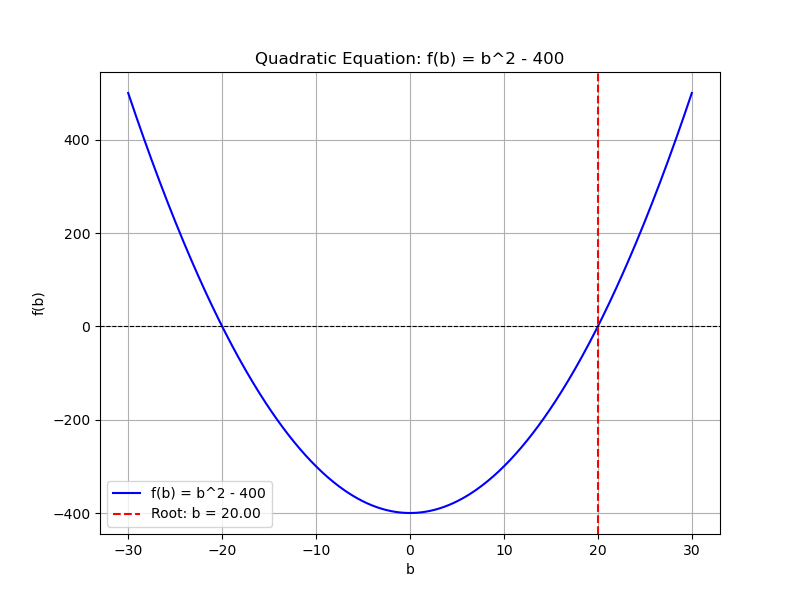
\includegraphics[width=0.5\textwidth]{figs/Figure_1.png} % Replace with your image file name
    \caption{A rectangular mango grove with length 40 m and breadth 20 m.}
    \label{fig:mango_grove}
\end{figure}
\end{document}
